\documentclass[10pt,a4paper]{article}
\usepackage[margin=0.8in]{geometry}
\usepackage{graphicx}
\usepackage{subcaption}
\usepackage{amsmath,amssymb}
\usepackage{float}
\usepackage{enumitem}
\usepackage{caption}
\captionsetup{font=small}
\setlength\parskip{4pt}
\setlength\parindent{0pt}

\title{COL783 Assignment 1 – Report}
\author{2023CS10807 Samyak Sanghvi \\ 2021CS50602 Kashish Goel\vspace{-0.8em}}
\date{\vspace{-1.5em}}

\begin{document}
\maketitle


\section{Part 1: Geometric Transformation}
\subsection{A. Method (Corner selection, rotation, homography)}
\textbf{Rotation (alignment).} Let the selected corners be $\{\mathbf{p}_i=(x_i,y_i)\}_{i=1}^4$ ordered $(\text{tl},\text{tr},\text{br},\text{bl})$. Define top and bottom midpoints
\[ \mathbf{m}_t=\tfrac{1}{2}(\mathbf{p}_{\text{tl}}+\mathbf{p}_{\text{tr}}),\qquad \mathbf{m}_b=\tfrac{1}{2}(\mathbf{p}_{\text{bl}}+\mathbf{p}_{\text{br}}), \]
the vector $\mathbf{v}=\mathbf{m}_b-\mathbf{m}_t$, and its angle $\theta=\operatorname{atan2}(v_y, v_x)$. To make the document vertical, rotate by $\alpha=\tfrac{\pi}{2}-\theta$ with
\[ R(\alpha)=\begin{bmatrix}\cos\alpha & -\sin\alpha\\ \sin\alpha & \cos\alpha\end{bmatrix}. \]
If $\mathbf{c}=(c_x,c_y)$ is the image center, the affine mapping is $\mathbf{x}' = R(\alpha)(\mathbf{x}-\mathbf{c})+\mathbf{c}$.

	\textbf{Perspective transform} A $3\times3$ transformation matrix (homography) $H$ maps homogeneous coordinates $\tilde{\mathbf{x}}=[x,y,1]^T$ to $\tilde{\mathbf{X}}=H\tilde{\mathbf{x}}$ with Cartesian $(X,Y)=(\tilde X/\tilde w,\tilde Y/\tilde w)$. With $H=[h_{ij}]$, each correspondence $(x,y)\mapsto(X,Y)$ satisfies
\[
 X = \frac{h_{11}x + h_{12}y + h_{13}}{h_{31}x + h_{32}y + h_{33}},\qquad
 Y = \frac{h_{21}x + h_{22}y + h_{23}}{h_{31}x + h_{32}y + h_{33}}.
\]
Four point pairs (the document corners to rectangle corners) give eight equations to solve $H$ up to scale. Warping uses the inverse mapping $\tilde{\mathbf{x}} \sim H^{-1}\tilde{\mathbf{X}}$ and resampling (nearest or bilinear).

\subsection{B. Results (Nearest vs Bilinear)}
	\textbf{Resampling formulas.} For a source location $(u,v)$ with $i=\lfloor u\rfloor$, $j=\lfloor v\rfloor$, $\alpha=u-i$, $\beta=v-j$:
\begin{itemize}[leftmargin=*]
  \item Nearest neighbour: $I'(X,Y)=I(\operatorname{round}(u),\operatorname{round}(v))$.
  \item Bilinear: $I'(X,Y)=(1-\alpha)(1-\beta)I_{i,j}+\alpha(1-\beta)I_{i+1,j}+(1-\alpha)\beta I_{i,j+1}+\alpha\beta I_{i+1,j+1}$.
\end{itemize}
\begin{figure}[H]
  \centering
  \begin{subfigure}[t]{.32\textwidth}
    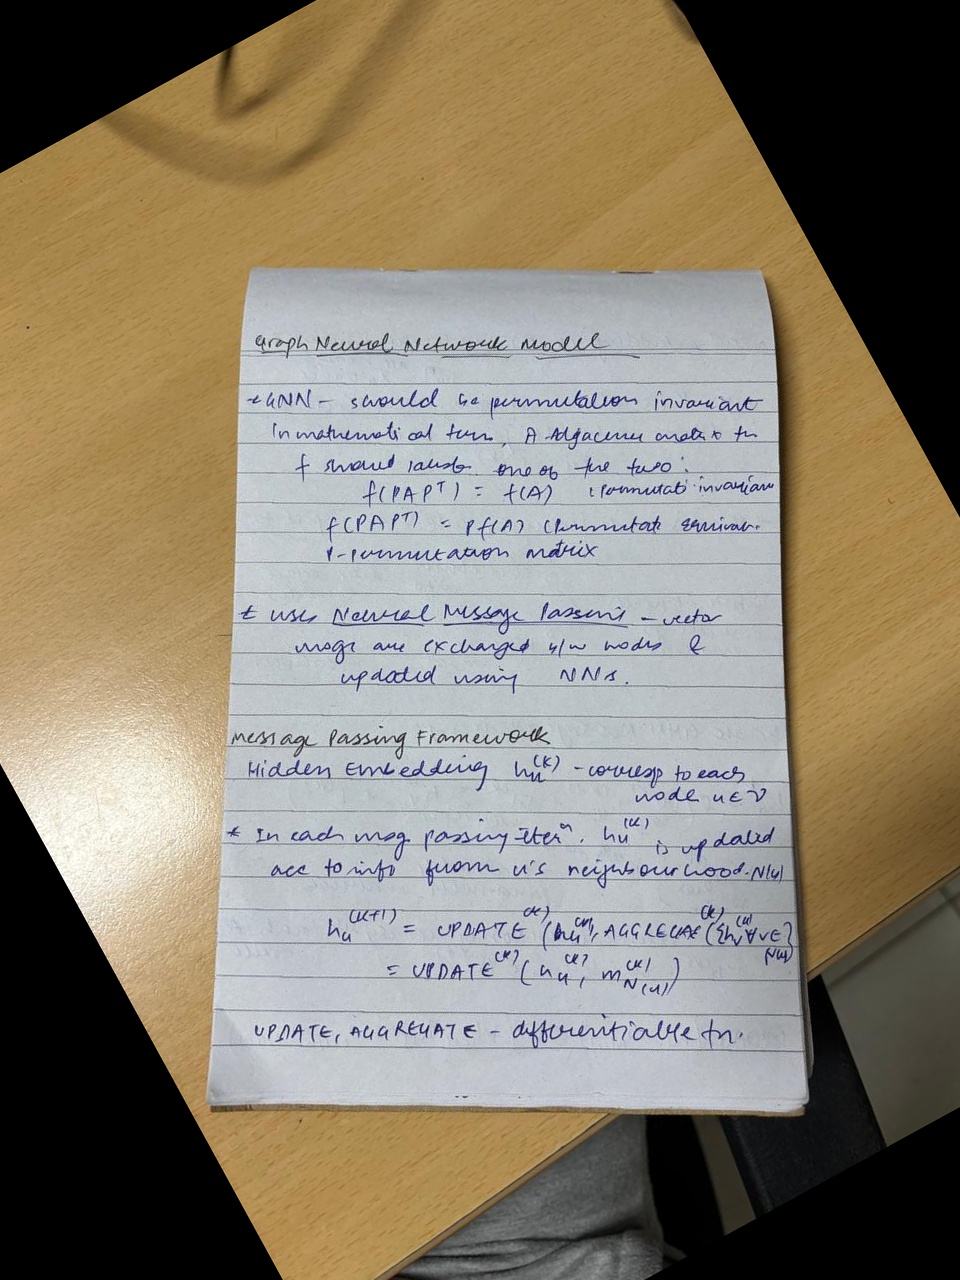
\includegraphics[width=\linewidth]{p1/results/rotated.jpg}
    \caption{Rotated}
  \end{subfigure}\hfill
  \begin{subfigure}[t]{.32\textwidth}
    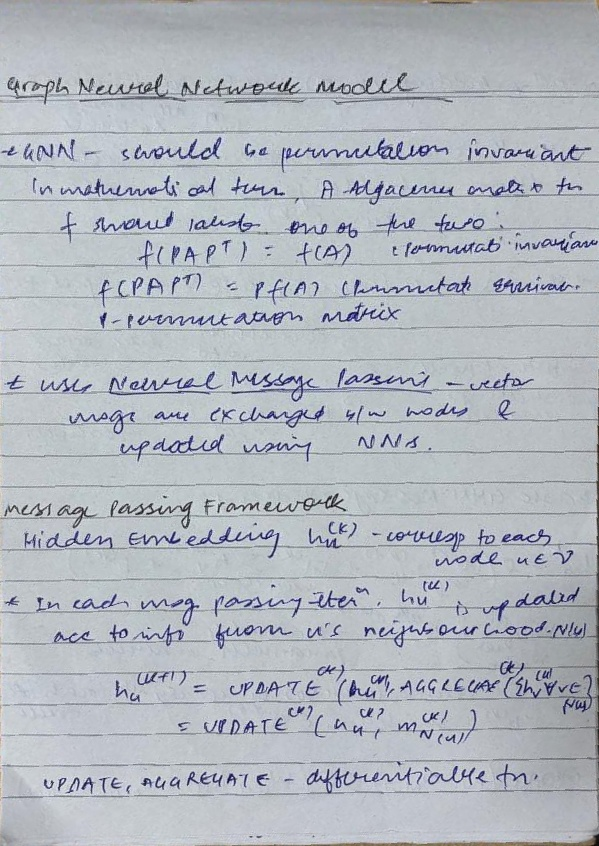
\includegraphics[width=\linewidth]{p1/results/scanned_nearest.jpg}
    \caption{Scanned (Nearest)}
  \end{subfigure}\hfill
  \begin{subfigure}[t]{.32\textwidth}
    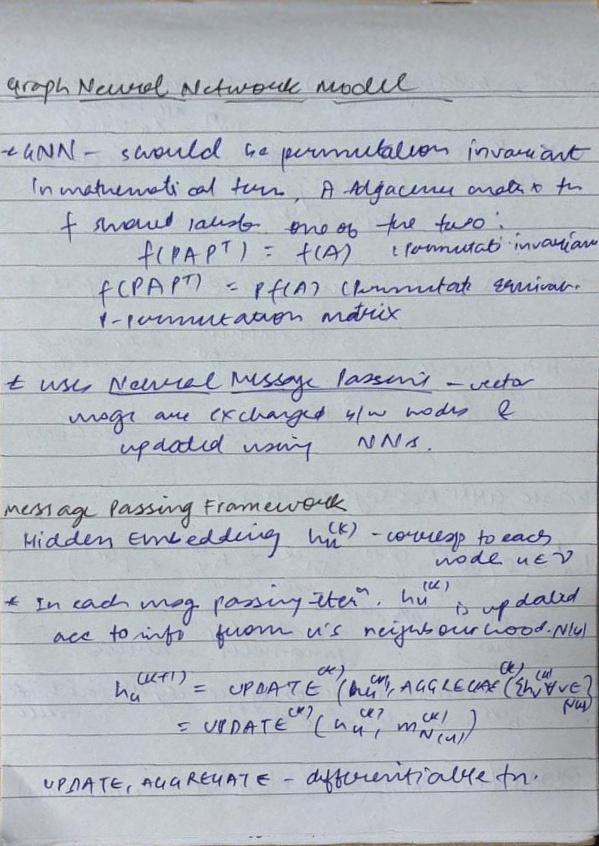
\includegraphics[width=\linewidth]{p1/results/scanned_bilinear.jpg}
    \caption{Scanned (Bilinear)}
  \end{subfigure}
  \caption{Part 1: Rotation and perspective transform with two interpolation schemes.}
\end{figure}
\vspace{-0.5em}
\noindent(Interpolation flags used in the code: \texttt{cv2.INTER\_NEAREST} for nearest-neighbour, \texttt{cv2.INTER\_LINEAR} for bilinear.)

\subsection{C. Zoomed comparisons}
	\textbf{Zoom crop.} The zoomed views are simple subimages: for height/width $200$, $I_{\text{zoom}}=I[0{:}200,\,0{:}200]$ (row, column slice).
\begin{figure}[H]
  \centering
  \begin{subfigure}[t]{.48\textwidth}
    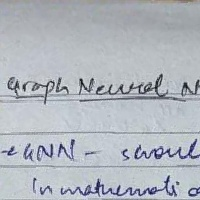
\includegraphics[width=\linewidth]{p1/results/zoom_nearest.jpg}
    \caption{Zoomed (Nearest)}
  \end{subfigure}\hfill
  \begin{subfigure}[t]{.48\textwidth}
    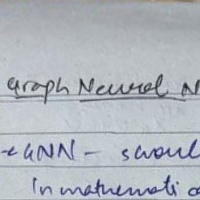
\includegraphics[width=\linewidth]{p1/results/zoom_bilinear.jpg}
    \caption{Zoomed (Bilinear)}
  \end{subfigure}
  \caption{Nearest is sharper but jaggy; bilinear is smoother with fewer aliasing artifacts.}
\end{figure}
\vspace{-0.5em}
\noindent(The zoom images are produced by cropping the top-left $200\times200$ pixels of the warped images in the code: \texttt{zoom = warped[:200,:200]}.)

\section{Part 2: Intensity Transformations}
All operations act on a grayscale image $I \in [0,255]$.

\subsection{A. Manual threshold}
Binary output $O=\mathbb{1}[I\ge T]\cdot 255$. Here $T=150$.
\begin{figure}[H]
  \centering
  \begin{subfigure}[t]{.32\textwidth}
    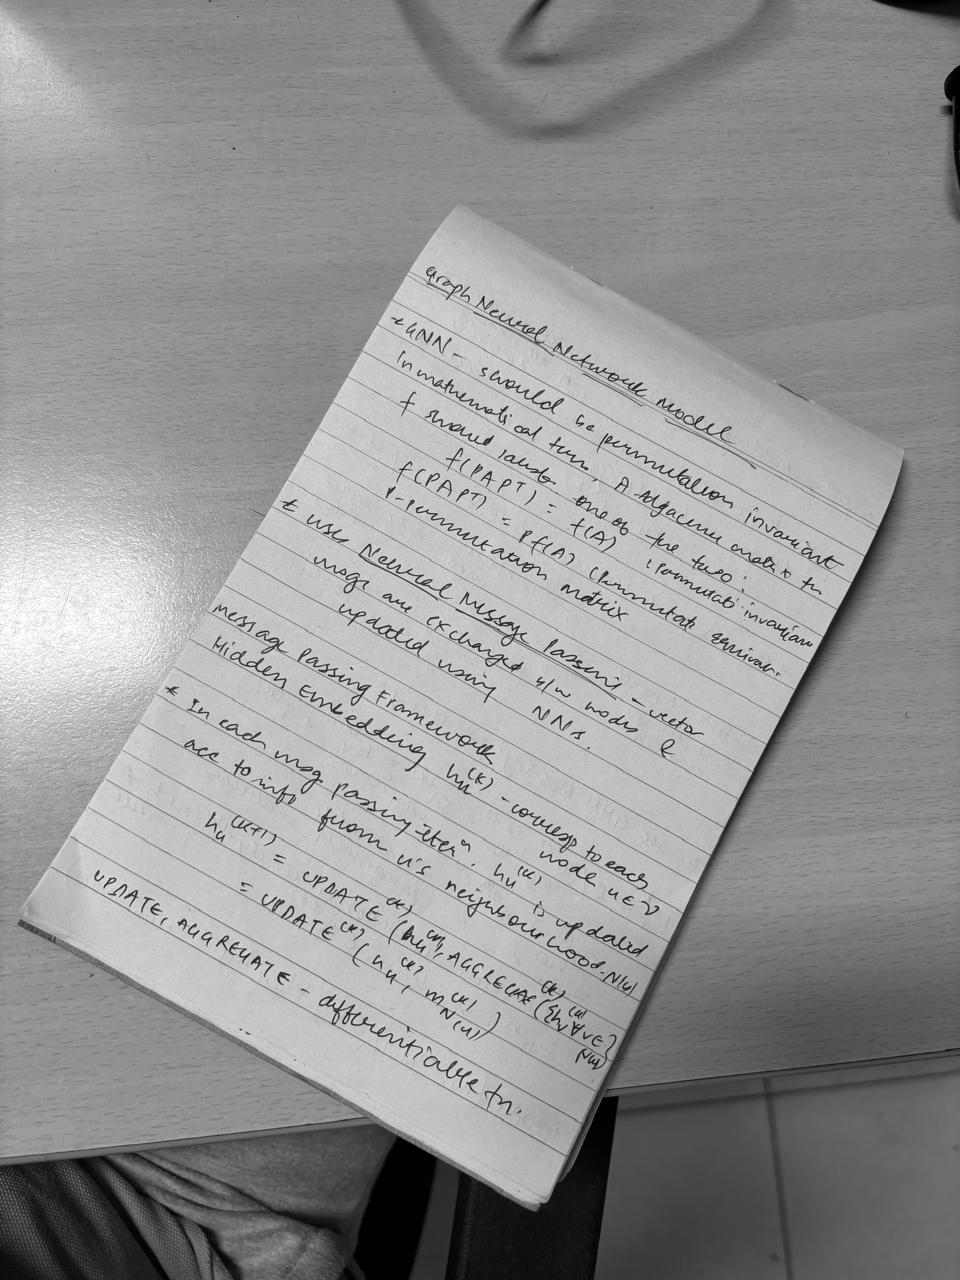
\includegraphics[width=\linewidth]{p2/results/image_orig_gray.png}
    \caption{Original}
  \end{subfigure}\hfill
  \begin{subfigure}[t]{.32\textwidth}
    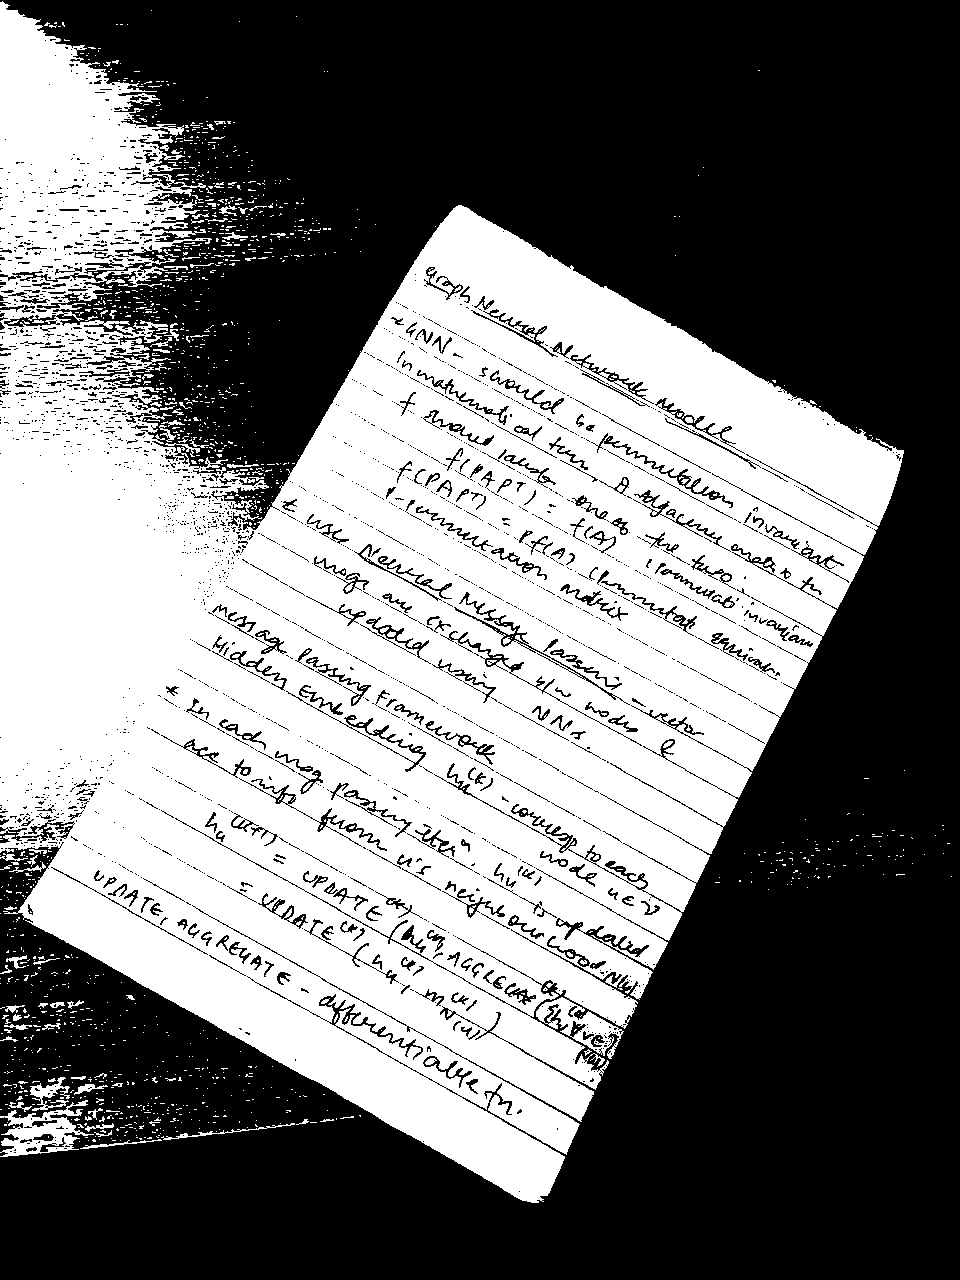
\includegraphics[width=\linewidth]{p2/results/image_manual_threshold_150.png}
    \caption{Threshold 150}
  \end{subfigure}\hfill
  \begin{subfigure}[t]{.32\textwidth}
    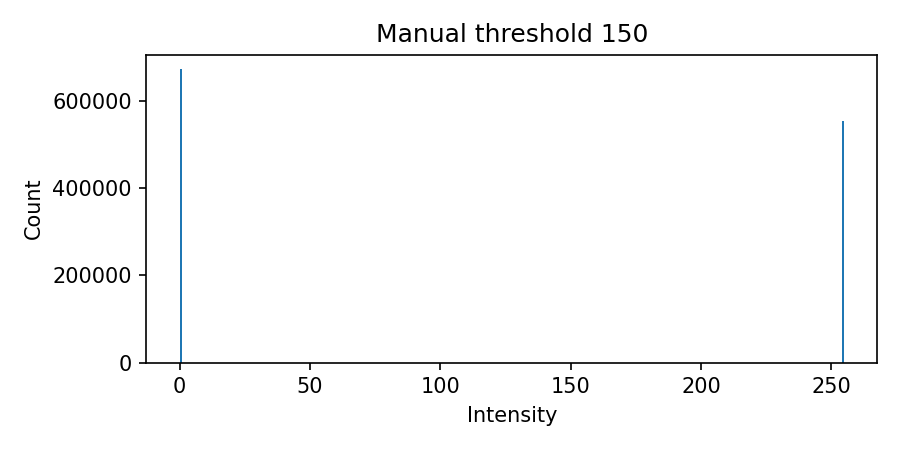
\includegraphics[width=\linewidth]{p2/results/image_hist_thr_manual.png}
    \caption{Histogram}
  \end{subfigure}
\end{figure}

\subsection{B. Linear transform}
Manual: $O=\mathrm{clip}(aI+b,0,255)$ with $a=1.9, b=-300$. Auto: percentiles map $[p_{\mathrm{low}},p_{\mathrm{high}}]\to[0,255]$.

\paragraph{Manual linear stretch.}
The linear transform rescales intensity via an affine mapping $I\mapsto aI+b$ followed by clipping to $[0,255]$. Increasing the slope $a>1$ increases contrast by spreading values away from mid-gray; the bias $b$ recenters the mapped values. For this image we found $(a,b)=(1.9,-300)$ by trial — this brightens the background (mapped toward 255) while pushing ink pixels toward 0, producing a near-binary visual appearance without explicit thresholding.

\paragraph{Automatic parameter selection (percentile-based contrast stretch).}
A robust automatic way to set $a$ and $b$ is to compute two percentiles of the input histogram, $p_{\mathrm{low}}$ and $p_{\mathrm{high}}$ (for example the 2nd and 98th percentiles), and linearly map that interval to $[0,255]$. Percentiles avoid extreme outliers (single very dark or very bright pixels) from dominating the stretch.

Given $p_{\mathrm{low}}$ and $p_{\mathrm{high}}$ (intensity values in $[0,255]$), compute
\[
a \;=\; \frac{255}{p_{\mathrm{high}}-p_{\mathrm{low}}},\qquad
b \;=\; -a \cdot p_{\mathrm{low}}.
\]
Then apply $O=\mathrm{clip}(aI+b,0,255)$.

\paragraph{Why percentiles?}
Using percentiles (instead of min and max) prevents a single speck of dirt or a specular highlight from forcing an extreme mapping that would crush contrast. The lower percentile sets a robust black reference; the upper percentile sets a robust white reference. Typical choices are $(p_{\mathrm{low}},p_{\mathrm{high}})=(2\%,98\%)$ or $(1\%,99\%)$; the exact choice trades off clipping more pixels (wider percentiles) vs. preserving extreme values (narrower percentiles).

\paragraph{Pseudocode (auto stretch)}
\begin{verbatim}
  # I is the grayscale image
  p_low  = percentile(I, p_low_percent)   # e.g., 2
  p_high = percentile(I, p_high_percent)  # e.g., 98
  if p_high == p_low:
      # fallback (flat image): use small slope or skip
  a = 255.0 / (p_high - p_low)
  b = -a * p_low
  O = clip(a * I + b, 0, 255).astype(uint8)
\end{verbatim}

\paragraph{Observed result.}
In our experiments the automatic percentile mapping (we used the 2nd and 98th percentiles in the provided figure c below) produces a clean separation of paper and ink while being robust to a few bright/dark outliers. Compared to the manual $(a,b)$ that was tuned visually, the percentile method gives a reproducible automatic result that generalizes across other page photographs.

\begin{figure}[H]
  \centering
  \begin{subfigure}[t]{.32\textwidth}
    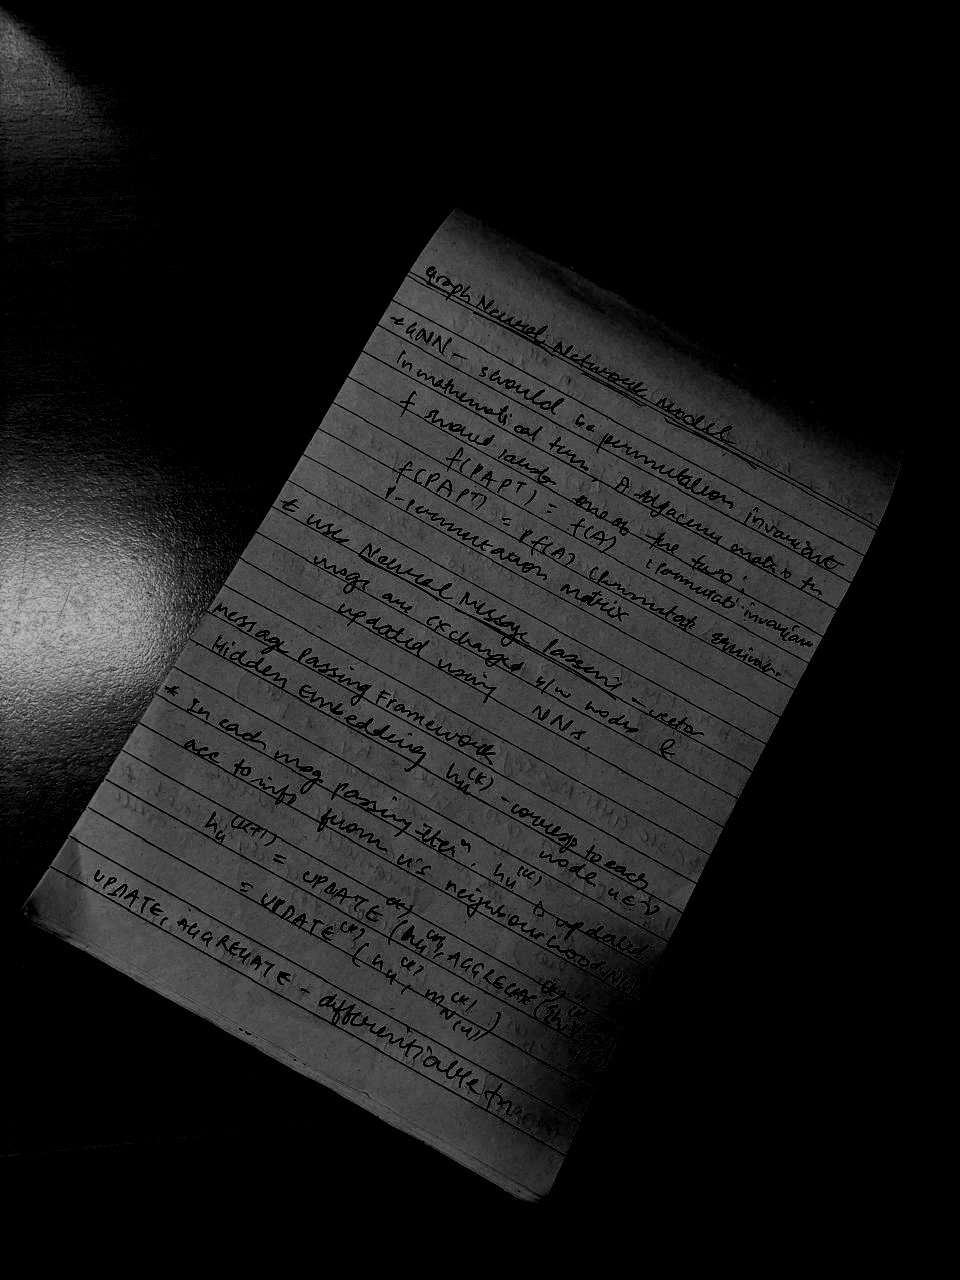
\includegraphics[width=\linewidth]{p2/results/image_linear_manual_a1.9_b-300.png}
    \caption{Manual $(a{=}1.9,b{=}{-}300)$}
  \end{subfigure}\hfill
  \begin{subfigure}[t]{.32\textwidth}
    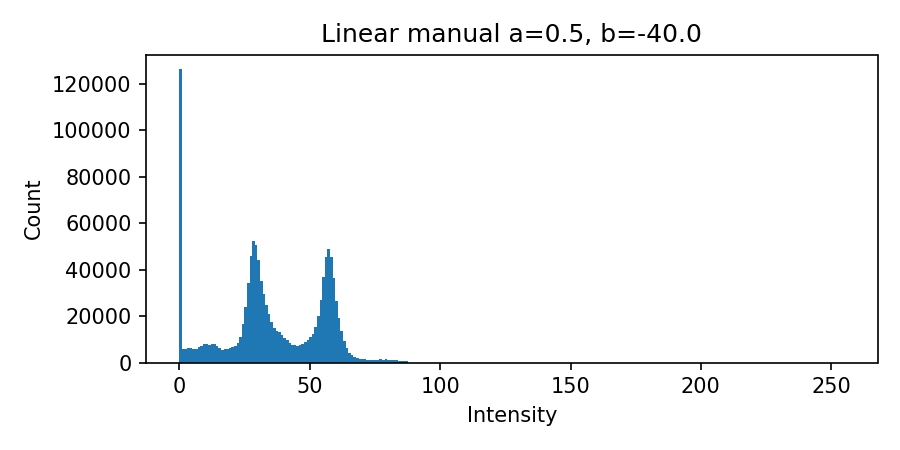
\includegraphics[width=\linewidth]{p2/results/image_hist_lin_manual.png}
    \caption{Histogram}
  \end{subfigure}\hfill
  \begin{subfigure}[t]{.32\textwidth}
    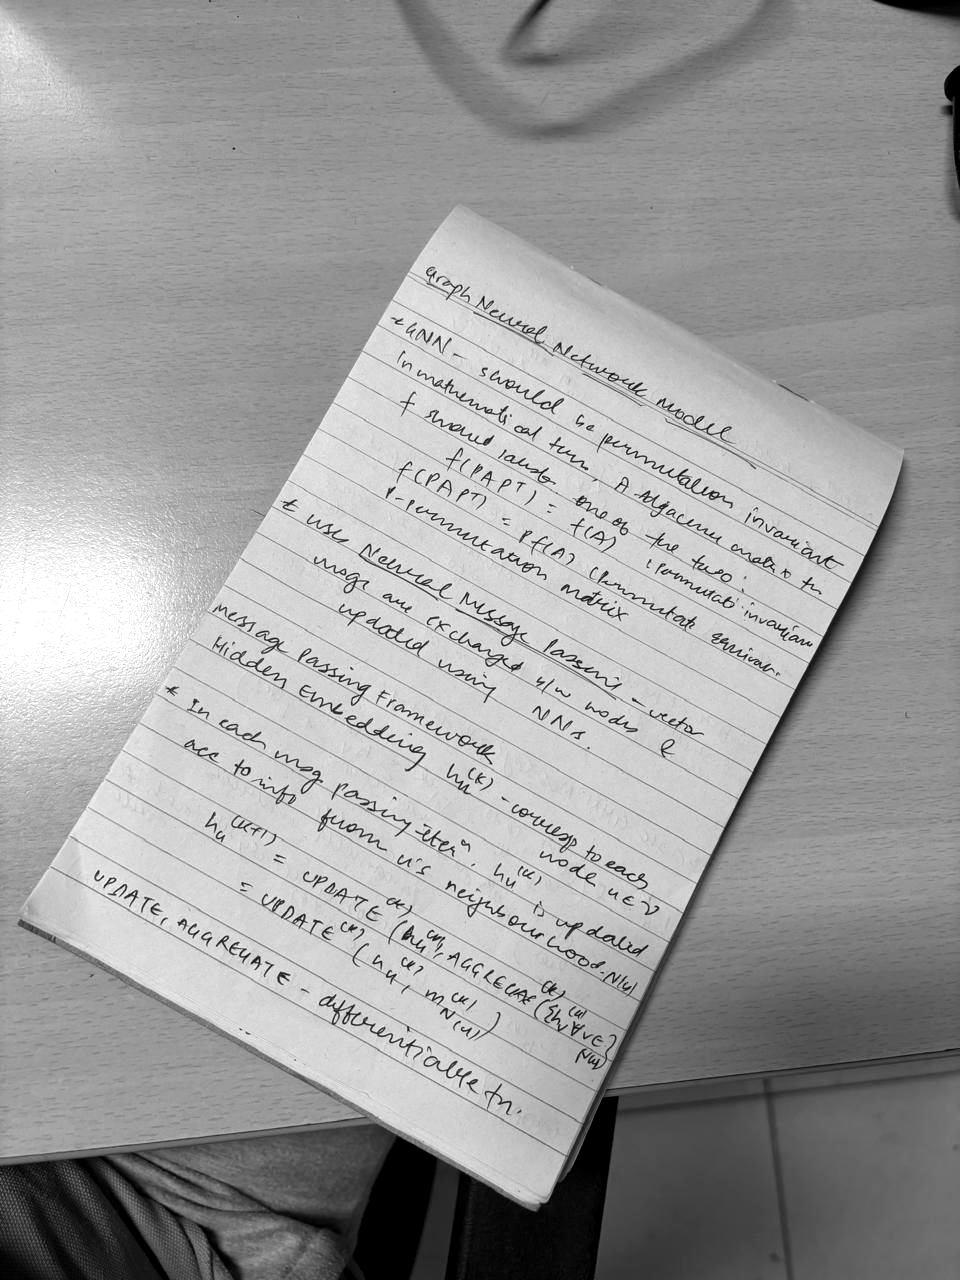
\includegraphics[width=\linewidth]{p2/results/image_linear_auto_pct2_98.png}
    \caption{Auto linear}
  \end{subfigure}
\end{figure}

\subsection{C. Gamma correction}
$O=255\,(I/255)^{\gamma}$. $\gamma{<}1$ brightens; $\gamma{>}1$ darkens.

\paragraph{Short explanation.}
Gamma correction applies the nonlinear mapping $O=255\,(I/255)^{\gamma}$. In our experiments (e.g. $\gamma=0.6$) gamma correction was used to enhance textual contrast in shadowed areas without fully clipping highlights; note it can also amplify noise, so it is most effective when combined with a subsequent contrast stretch or denoising step.

\begin{figure}[H]
  \centering
  \begin{subfigure}[t]{.32\textwidth}
    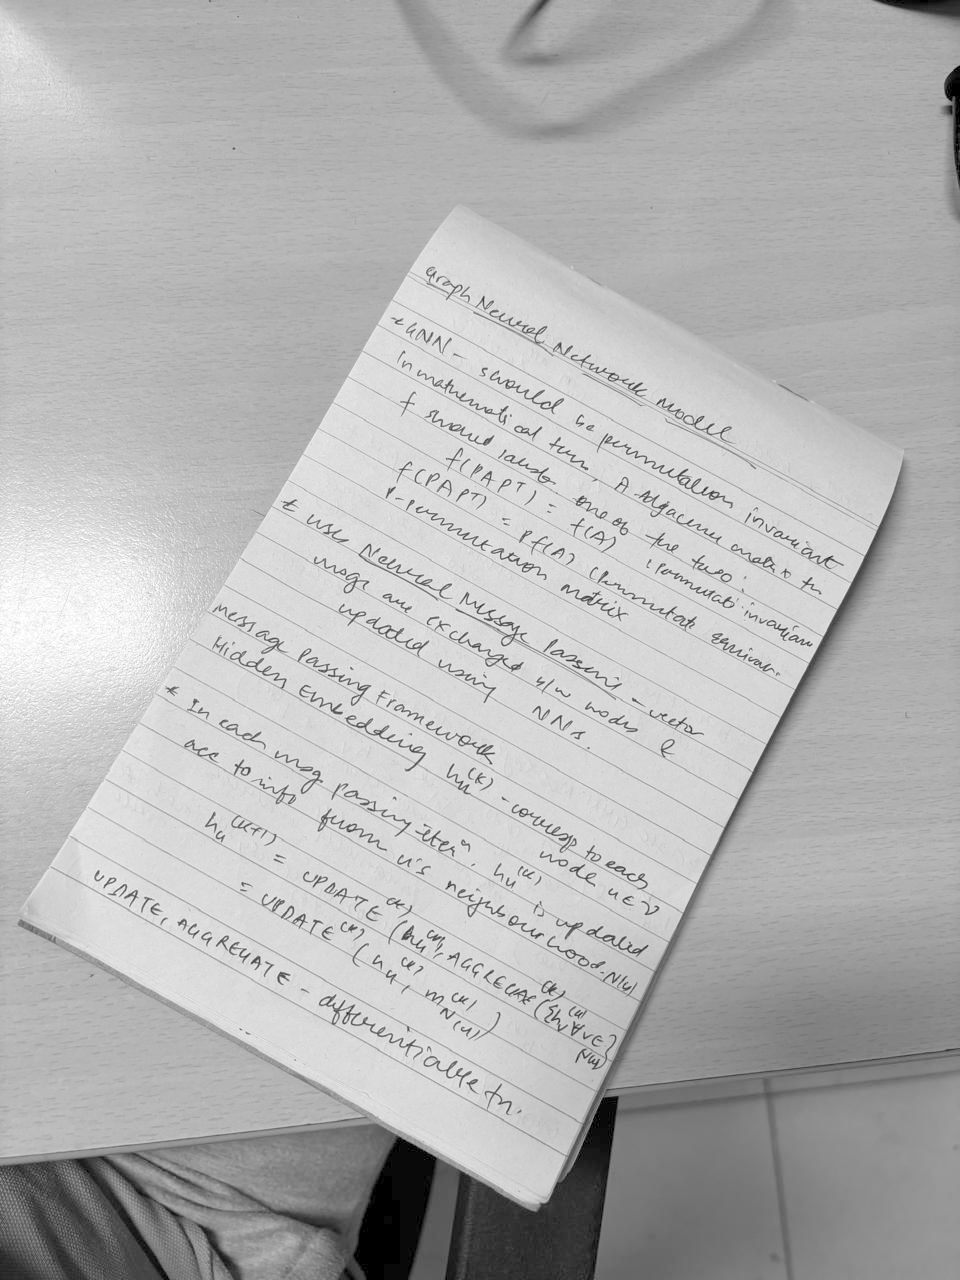
\includegraphics[width=\linewidth]{p2/results/image_gamma_0.60.png}
    \caption{$\gamma=0.6$}
  \end{subfigure}\hfill
  \begin{subfigure}[t]{.32\textwidth}
    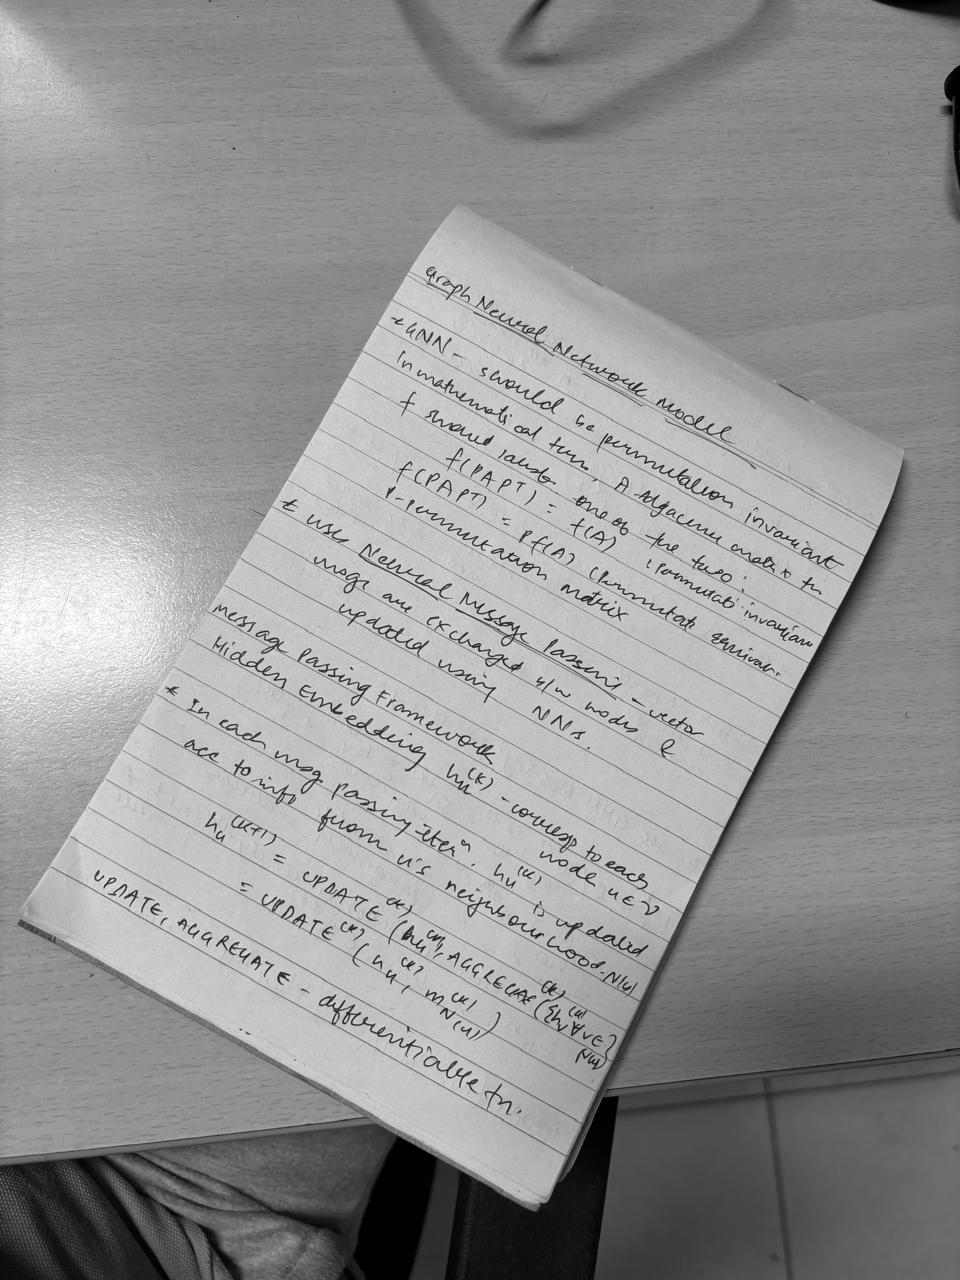
\includegraphics[width=\linewidth]{p2/results/image_gamma_1.00.png}
    \caption{$\gamma=1.0$}
  \end{subfigure}\hfill
  \begin{subfigure}[t]{.32\textwidth}
    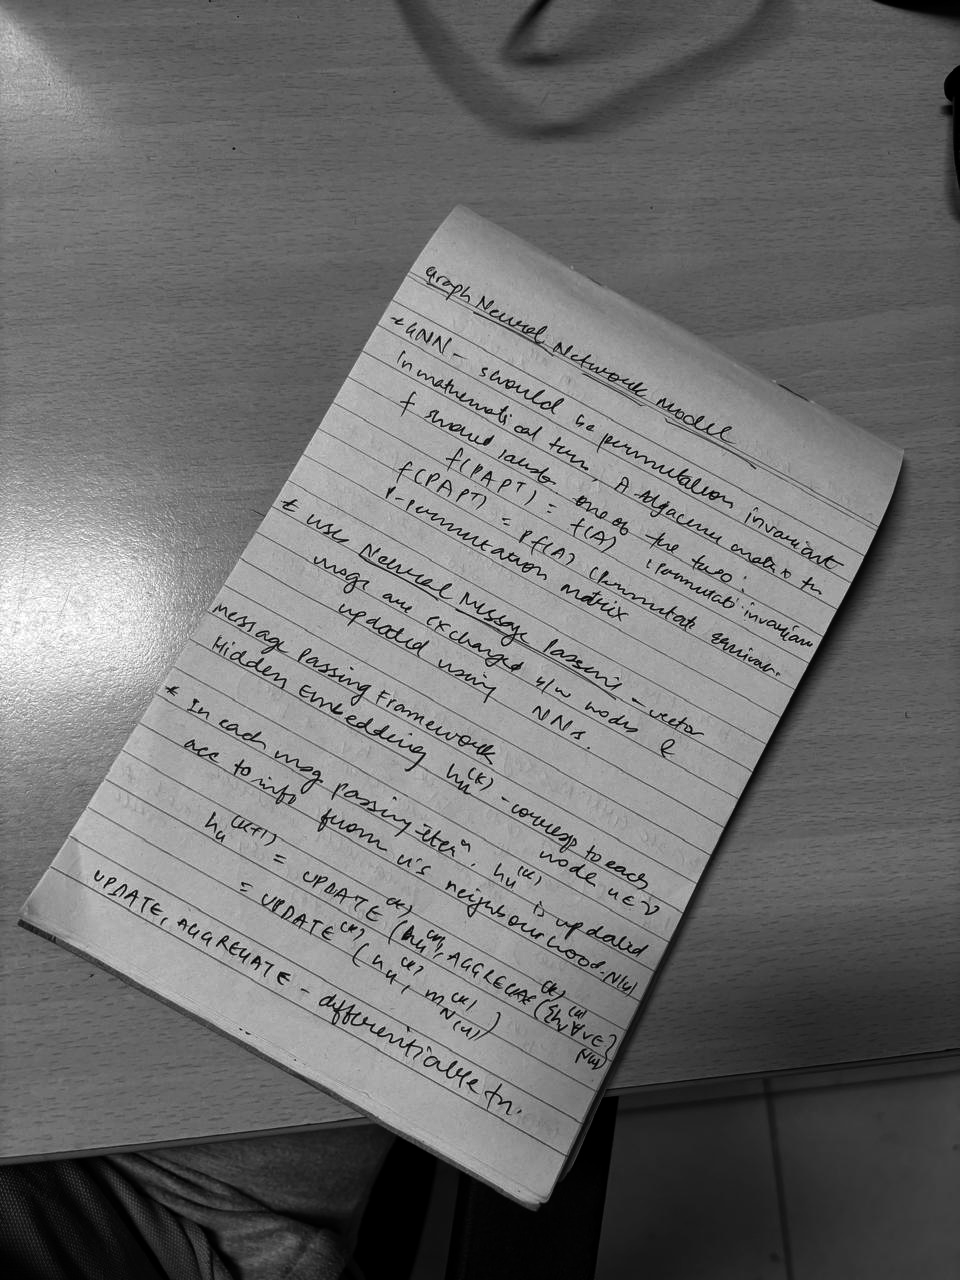
\includegraphics[width=\linewidth]{p2/results/image_gamma_1.60.png}
    \caption{$\gamma=1.6$}
  \end{subfigure}
\end{figure}

\subsection{D. Histogram equalization}
Spreads intensities to use full range; see histogram flattening effect.

\paragraph{Observed result on our image.}
Comparing original histogram and equalized histogram. The original histogram shows two dominant modes (background and ink) with additional midtones caused by lighting variations. After equalization the intensities are spread, but the result remains strongly non-uniform: two prominent peaks appear at new intensity locations and the histogram shows tall, narrow spikes with many empty bins in between. In visual terms this means that equalization redistributed intensities but did not produce a clean white paper + black text separation; instead it amplified mid-level variations and introduced contrast artifacts in some regions.

\begin{figure}[H]
  \centering
  \begin{subfigure}[t]{.32\textwidth}
    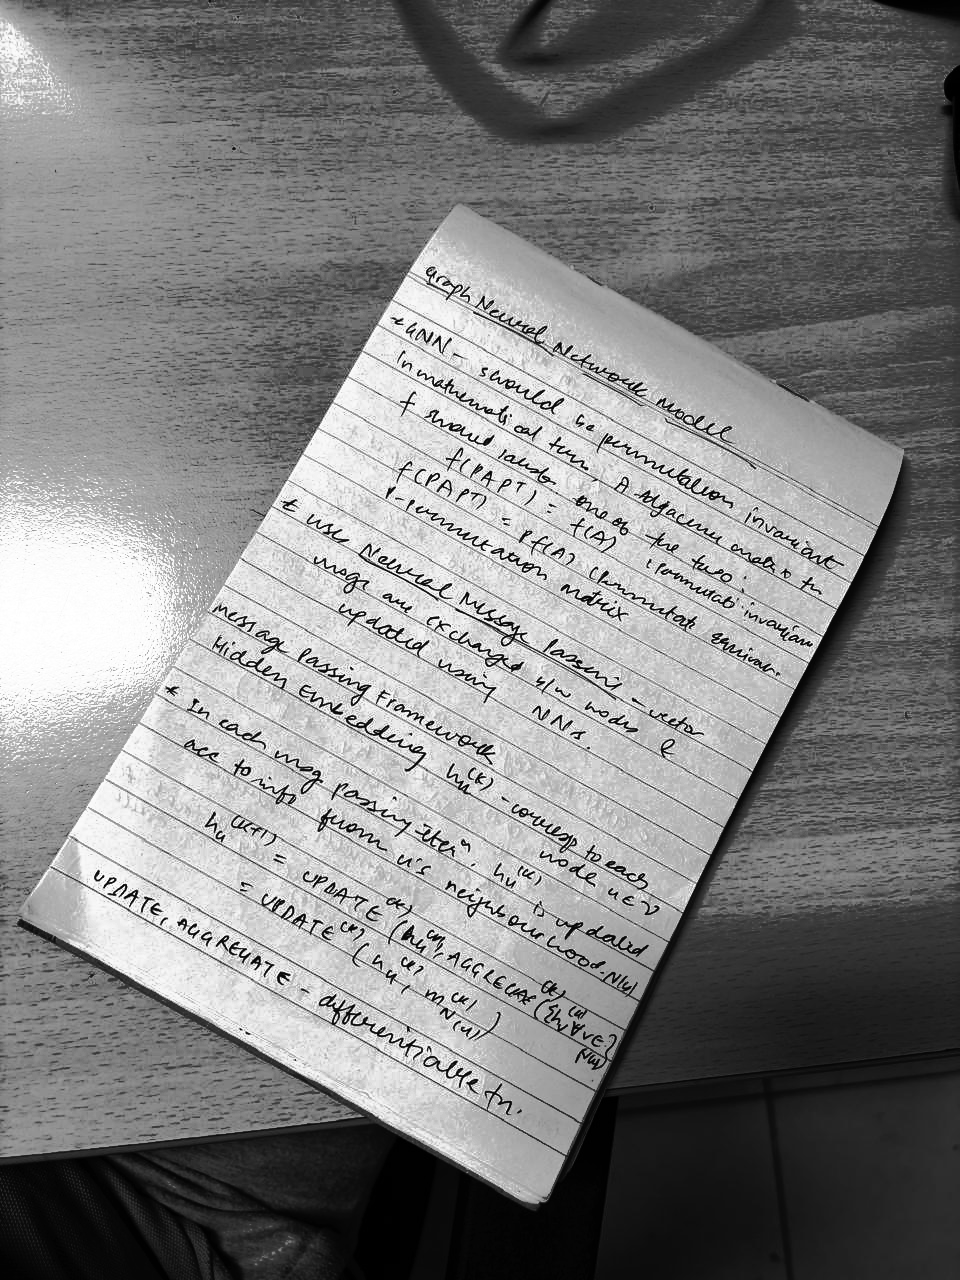
\includegraphics[width=\linewidth]{p2/results/image_histeq.png}
    \caption{Equalized}
  \end{subfigure}\hfill
  \begin{subfigure}[t]{.32\textwidth}
    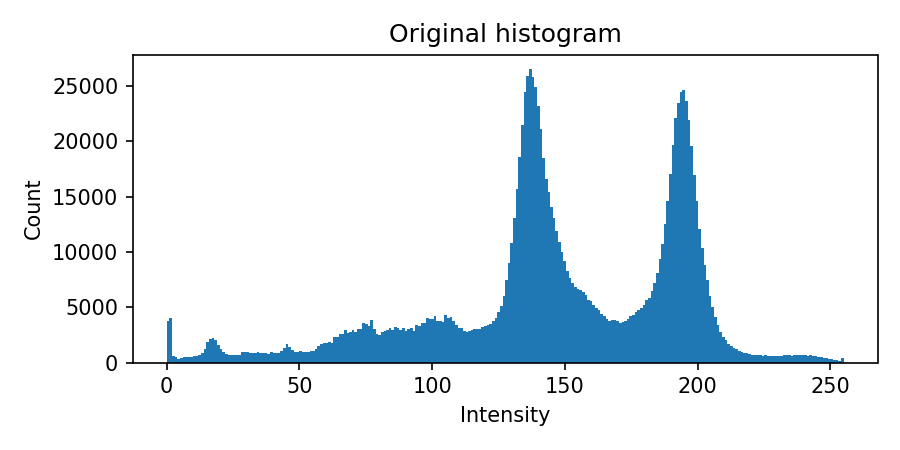
\includegraphics[width=\linewidth]{p2/results/image_hist_orig.png}
    \caption{Original hist}
  \end{subfigure}\hfill
  \begin{subfigure}[t]{.32\textwidth}
    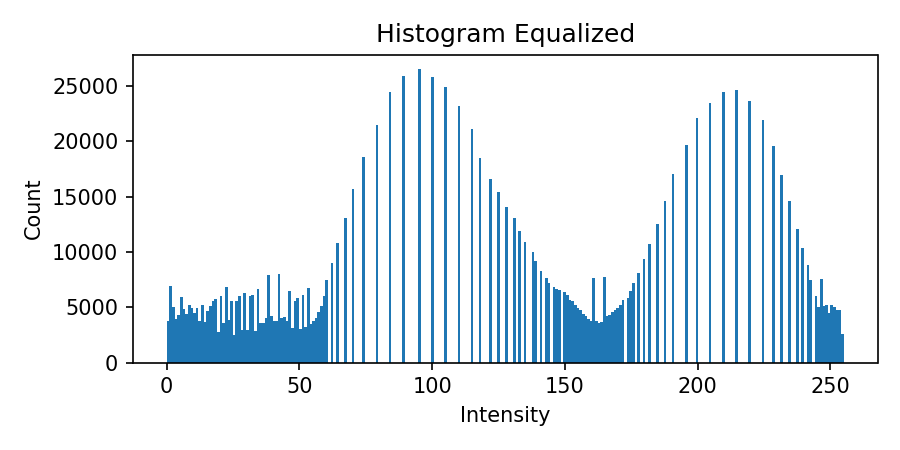
\includegraphics[width=\linewidth]{p2/results/image_hist_histeq.png}
    \caption{Equalized hist}
  \end{subfigure}
\end{figure}

\section{Part 3: Watermarking}
\subsection{A. Mask extraction}
The IITD logo is binarized using a high threshold to obtain a mask $M\in\{0,1\}$ aligned with the logo.
\begin{figure}[H]
  \centering
  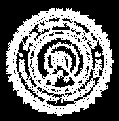
\includegraphics[width=.45\textwidth]{p3/results/logo_mask.jpg}
  \caption{Binary mask of the logo region.}
\end{figure}

\subsection{B. Blending (50\% transparency)}
With document $D$, logo $L$, mask $M$: $O = D + 0.5\,M\,(L-D) = (1-0.5M)D + 0.5M\,L$.
\begin{figure}[H]
  \centering
  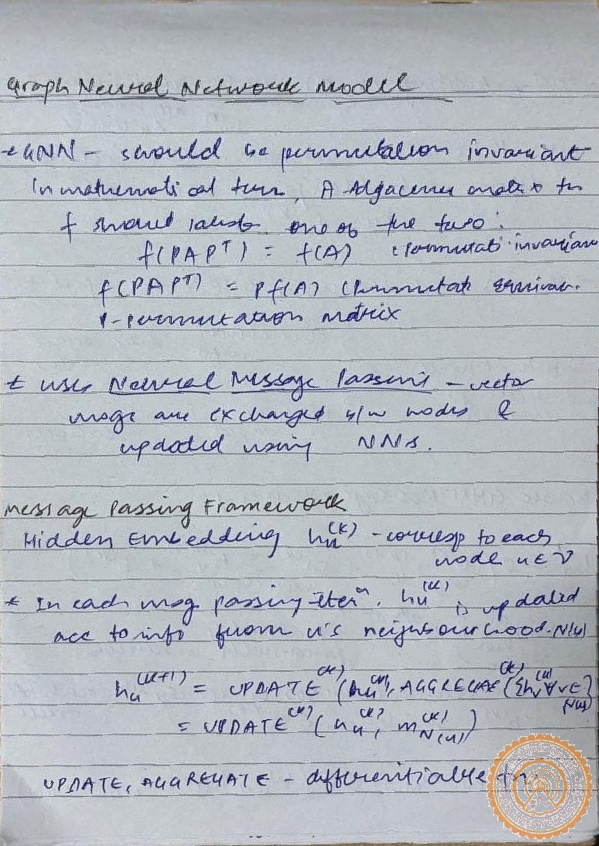
\includegraphics[width=.6\textwidth]{p3/results/watermarked.jpg}
  \caption{Final watermarked image with 50\% transparency.}
\end{figure}

\section{Part 4: HDR Histogram Equalization}
\subsection{A. Algorithm}
We equalize HDR intensities without pre-quantization by mapping each channel via its empirical CDF $F$:
\[ s = a + (b-a)\,F(r), \quad \text{with } a{=}0,\; b{=}256. \]
Implementation uses sorting and rank-based CDF with linear interpolation to preserve order and avoid banding.
\begin{figure}[H]
  \centering
  \begin{subfigure}[t]{.48\textwidth}
    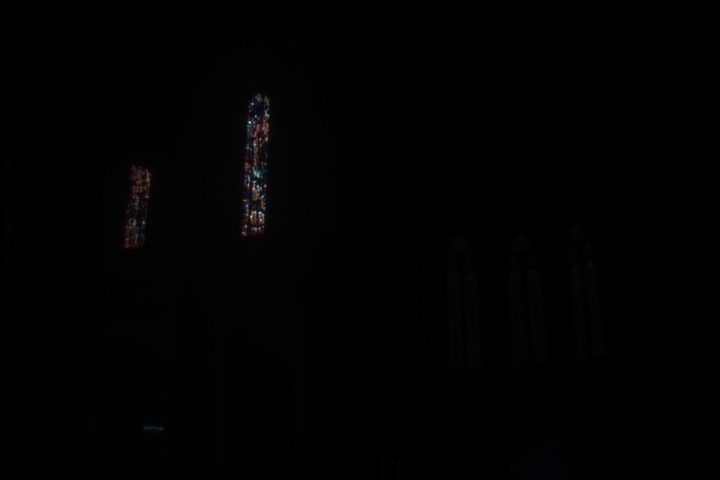
\includegraphics[width=\linewidth]{p4/results/hdr_original.jpg}
    \caption{Original (tonemapped for view)}
  \end{subfigure}\hfill
  \begin{subfigure}[t]{.48\textwidth}
    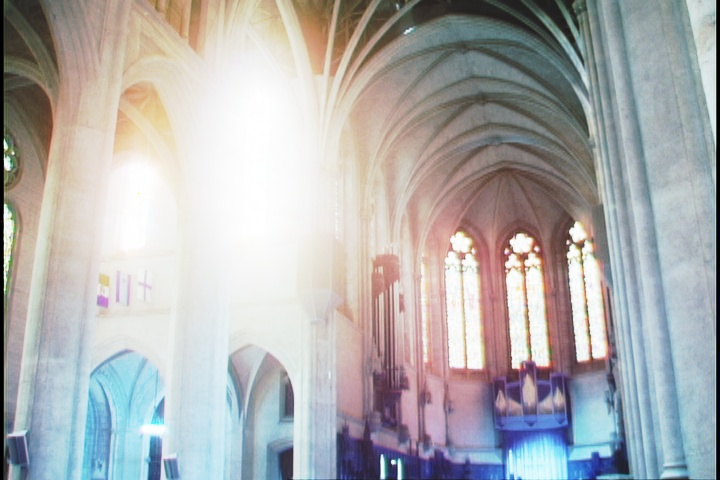
\includegraphics[width=\linewidth]{p4/results/hdr_equalized.jpg}
    \caption{After equalization}
  \end{subfigure}
\end{figure}

\subsection{B. Demonstration (mapping to $[0,255]$)}
Each channel is transformed by $T(r)=a+(b-a)F(r)$ with $(a,b)=(0,256)$. Since $0\le F(r)\le 1$, it follows that $0\le T(r)<256$. When rendering to 8-bit, values are clipped/quantized to $\{0,\ldots,255\}$. The outputs in Fig.4(b) visually confirm improved contrast while respecting the target range.

\subsection{C. Proofs}
	\textbf{Setup.} Let $R$ be a real-valued intensity random variable with (possibly channel-wise) CDF $F_R(r)=\mathbb{P}(R\le r)$. Define the equalization map on $[a,b)$ by
\[ T(r)=a+(b-a)\,F_R(r). \]

	\textbf{(C1) Idempotence.} Let $S=T(R)$. For $s\in[a,b)$,
\[ \mathbb{P}(S\le s)=\mathbb{P}\big(F_R(R)\le \tfrac{s-a}{b-a}\big)=\tfrac{s-a}{b-a}, \]
so $S$ is uniform on $[a,b)$. Its CDF is $F_S(s)=(s-a)/(b-a)$. Equalizing $S$ gives
\[ T'(s)=a+(b-a)F_S(s)=a+(b-a)\tfrac{s-a}{b-a}=s, \]
thus applying histogram equalization twice yields the identity (no further change). The same argument holds for empirical equalization: the map is a (scaled) rank transform, and applying the rank transform to already uniform ranks is the identity.

	\textbf{(C2) Invariance under strictly increasing transforms.} Let $g:\mathbb{R}\to\mathbb{R}$ be strictly increasing and define $Z=g(R)$. Then for any $x$,
\[ F_Z(x)=\mathbb{P}(g(R)\le x)=\mathbb{P}(R\le g^{-1}(x))=F_R\big(g^{-1}(x)\big). \]
Equalizing $Z$ at input value $z=g(r)$ yields
\[ T_g(z)=a+(b-a)\,F_Z(z)=a+(b-a)\,F_R\big(g^{-1}(g(r))\big)=a+(b-a)\,F_R(r)=T(r). \]
Hence, equalizing after any strictly increasing intensity transform produces the same result as equalizing the original image. In the empirical (discrete) case, $g$ preserves order, so ranks---and therefore the equalized outputs---are identical up to ties.

\section{Part 5: Convolution}
\subsection{A. Laplacian (edge emphasis)}
Using kernel 
\[
\begin{bmatrix}
0 & 1 & 0 \\
1 & -4 & 1 \\
0 & 1 & 0
\end{bmatrix}
\]
with additive constant $c{=}128$ for visualization. 
The convolution was implemented with \textbf{zero-padding} (i.e.\ pixels outside the image are treated as zero). 
This ensures that the output has the same spatial dimensions as the input image.

\begin{figure}[H]
  \centering
  \begin{subfigure}[t]{.48\textwidth}
    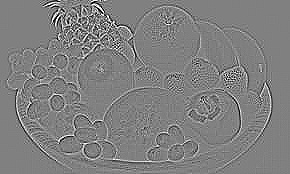
\includegraphics[width=\linewidth]{p5/results/download_lap.jpg}
    \caption{Laplacian + 128}
  \end{subfigure}\hfill
  \begin{subfigure}[t]{.48\textwidth}
    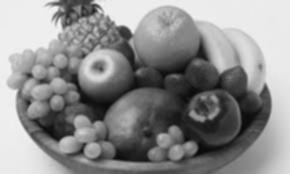
\includegraphics[width=\linewidth]{p5/results/download_mean.jpg}
    \caption{Mean 3\,\texttimes\,3 (reference smoothing)}
  \end{subfigure}
\end{figure}

\subsection{B. Gaussian: naive 2D vs separable 1D+1D}
Gaussian smoothing was tested with $\sigma=2$. 
The naive implementation uses a full 2D kernel, while the separable method applies two 1D kernels sequentially (horizontal + vertical). 
Separability reduces computational complexity from $\mathcal{O}(k^2)$ per pixel to $\mathcal{O}(2k)$. 

Both results are visually equivalent
but the timing confirms the efficiency gain:
\[
\text{Naive 2D runtime: 1565.02 ms, \quad Separable runtime: 283.40 ms}
\]

\begin{figure}[H]
  \centering
  \begin{subfigure}[t]{.48\textwidth}
    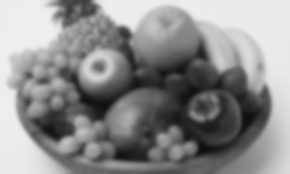
\includegraphics[width=\linewidth]{p5/results/gauss_naive_sigma2.0.jpg}
    \caption{Naive 2D ($\sigma=2$)}
  \end{subfigure}\hfill
  \begin{subfigure}[t]{.48\textwidth}
    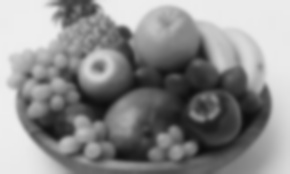
\includegraphics[width=\linewidth]{p5/results/gauss_sep_sigma2.0.jpg}
    \caption{Separable ($\sigma=2$)}
  \end{subfigure}
\end{figure}

\subsection{C. Laplacian of Gaussian (three ways)}
We computed the Laplacian of Gaussian (LoG) in three mathematically equivalent ways:
\begin{enumerate}
    \item $(L*G)*f$ : convolving Laplacian and Gaussian kernels first, then applying to $f$,
    \item $L*(G*f)$ : Gaussian smoothing followed by Laplacian,
    \item $G*(L*f)$ : Laplacian first, then Gaussian smoothing.
\end{enumerate}

Due to discrete padding and rounding to 8-bit values, the three results differ slightly in practice. 
Theoretically they coincide in the continuous, infinite-domain case.

Hence, the convolved kernel looks slightly different from the other two methods, which involve intermediate results that are clipped/rounded.

\begin{figure}[H]
  \centering
  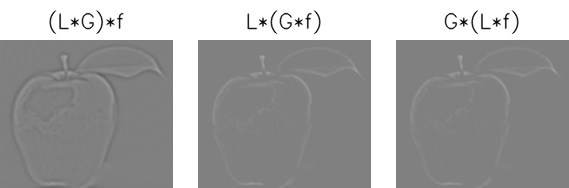
\includegraphics[width=.98\textwidth]{p5/results/log_combined_labeled.jpg}
  \caption{Three LoG variants, laid out with labels.}
\end{figure}

\section{Part 6: Intensity Transform vs Convolution}
\subsection{A. Linear case}
Let $T(r)=a r + b$ and let $w$ be any convolution kernel (not necessarily summing to 1). Define
\[ T'(r) = a\,r + b\,S, \qquad S = \sum_{x,y} w(x,y). \]
Then
\[ T'(w*f) = a\,(w*f) + b\,S = w*(a f) + b\sum w = w*(a f + b) = w*T(f). \]
Thus $T'(w*f)=w*T(f)$ holds for all $a,b$ and any $w$ with finite sum $S$. We verify this numerically in p6 (see images below).

\begin{figure}[H]
  \centering
  \begin{subfigure}[t]{.48\textwidth}
    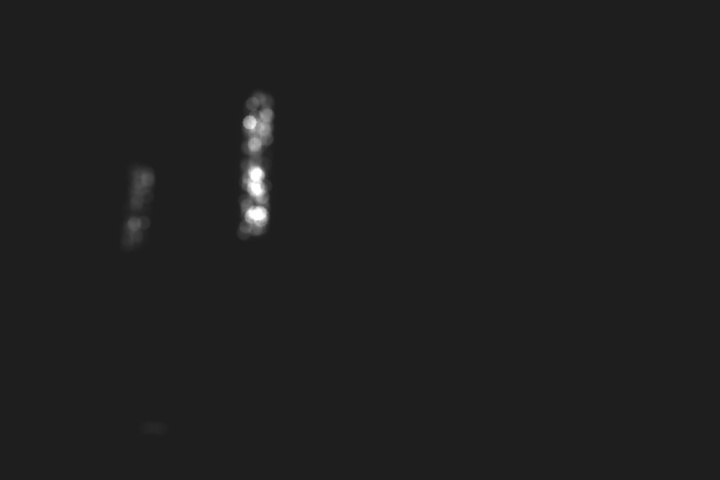
\includegraphics[width=\linewidth]{p6/results/p6_6a_wTf.jpg}
    \caption{$w*T(f)$}
  \end{subfigure}\hfill
  \begin{subfigure}[t]{.48\textwidth}
    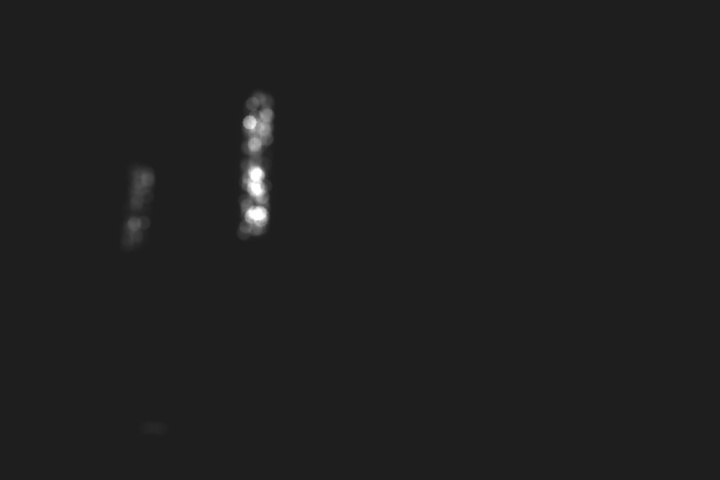
\includegraphics[width=\linewidth]{p6/results/p6_6a_Tp_wf.jpg}
    \caption{$T'(w*f)$}
  \end{subfigure}
  \caption{Part 6A: Linear case equivalence demonstrated on the HDR image.}
\end{figure}

\subsection{B. Nonlinear gamma vs blur}
Take $T$ to be gamma with rescaling to [0,1], i.e., $T(r)= (r')^{\gamma}$ after robust normalization $r'\in[0,1]$. Let $w$ be a normalized disk kernel of radius $r$ (sum to 1). We compare
\[ \text{Gamma}\to\text{Blur}:\;\; w * T(f) \quad\text{vs}\quad \text{Blur}\to\text{Gamma}:\;\; T(w*f). \]
Because gamma is nonlinear, $w*T(f)\ne T(w*f)$ in general. Blurring first (then compressing dynamic range) tends to mimic an out-of-focus capture, whereas gamma first can preserve micro-contrast before blur. Empirically, the blur-then-gamma result appears closer to an optically defocused image.

\begin{figure}[H]
  \centering
  \begin{subfigure}[t]{.32\textwidth}
    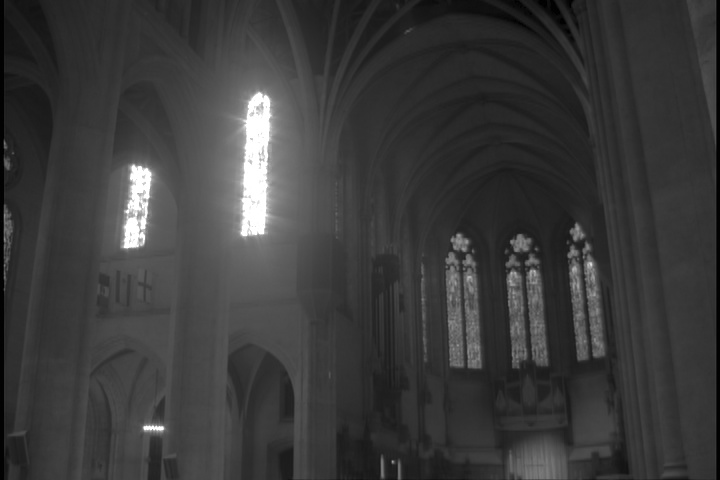
\includegraphics[width=\linewidth]{p6/results/p6_gamma.jpg}
    \caption{Gamma only}
  \end{subfigure}\hfill
  \begin{subfigure}[t]{.32\textwidth}
    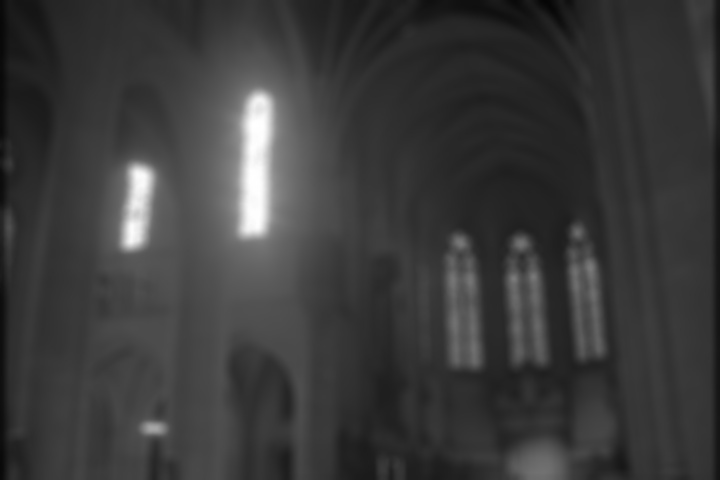
\includegraphics[width=\linewidth]{p6/results/p6_gamma_then_blur.jpg}
    \caption{$w*T(f)$ (Gamma then Blur)}
  \end{subfigure}\hfill
  \begin{subfigure}[t]{.32\textwidth}
    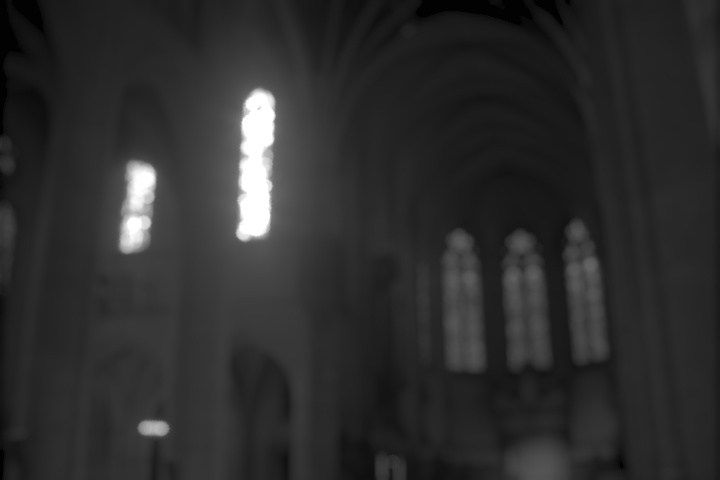
\includegraphics[width=\linewidth]{p6/results/p6_blur_then_gamma.jpg}
    \caption{$T(w*f)$ (Blur then Gamma)}
  \end{subfigure}
  \caption{Part 6B: Nonlinear order-of-operations comparison.}
\end{figure}

\section{Part 7: Color slicing / HSI}
\subsection{A. HSI channels}
We convert the input RGB image into an HSI color space and display the three channels separately.

\begin{figure}[H]
  \centering
  \begin{subfigure}[t]{.32\textwidth}
    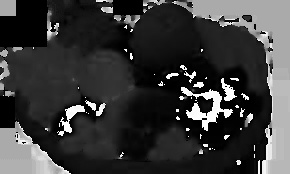
\includegraphics[width=\linewidth]{p7/results/hue_channel.jpg}
    \caption{Hue}
  \end{subfigure}\hfill
  \begin{subfigure}[t]{.32\textwidth}
    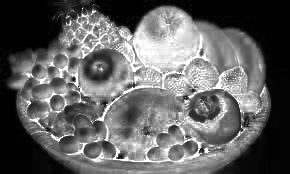
\includegraphics[width=\linewidth]{p7/results/saturation_channel.jpg}
    \caption{Saturation}
  \end{subfigure}\hfill
  \begin{subfigure}[t]{.32\textwidth}
    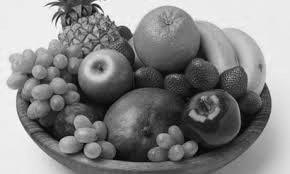
\includegraphics[width=\linewidth]{p7/results/intensity_channel.jpg}
    \caption{Intensity}
  \end{subfigure}
\end{figure}

\subsection{B. Masks and comparison}

\paragraph{Colour-slicing principle.}
Colour slicing selects pixels whose colour vectors lie within a cuboid (or hyperbox) centred at a chosen seed colour. We implement this in two spaces:

\begin{enumerate}
  \item \textbf{RGB cuboid:} select pixels $p=(R,G,B)$ such that $|R-R_s|\le \Delta_R$, $|G-G_s|\le\Delta_G$, $|B-B_s|\le\Delta_B$.
  \item \textbf{HSI cuboid (practical variant):} select pixels for which:
    \begin{itemize}
      \item Angular hue distance $d_H=\min(|H-H_s|,360^\circ-|H-H_s|)\le\Delta_H$,
      \item Saturation $|S-S_s|\le\Delta_S$,
      \item Intensity $|I-I_s|\le\Delta_I$ (optional).
    \end{itemize}
\end{enumerate}

\paragraph{Pseudocode (mask creation).}
\begin{verbatim}
  # seed = pixel at chosen seed location
  # For RGB mask:
  mask_rgb = (abs(R - seed.R) <= dR) &
             (abs(G - seed.G) <= dG) &
             (abs(B - seed.B) <= dB)

  # For HSI mask:
  # compute angular hue distance:
  dh = abs(H - seed.H)
  dh = min(dh, 360 - dh)
  mask_hsi = (dh <= dH) & (abs(S - seed.S) <= dS)
  # optionally refine with intensity:
  mask_hsi = mask_hsi & (abs(I - seed.I) <= dI)
\end{verbatim}

\paragraph{Comparison (observed behaviour).}
\begin{itemize}
  \item \textbf{RGB mask} is simple but sensitive to intensity variations: shadows, highlights, and shading change RGB channels and may cause holes or false positives.
  \item \textbf{HSI mask} better isolates chromaticity and is therefore more robust to brightness changes. However, it can fail where saturation is low (pale regions of the object appear grey and are missed).
  \item In practice we found the HSI-based mask to include more of the coloured object while excluding background; small gaps near shadowed regions were fixed by relaxing $\Delta_I$ or performing a small morphological closing.
\end{itemize}

\begin{figure}[H]
  \centering
  \begin{subfigure}[t]{.48\textwidth}
    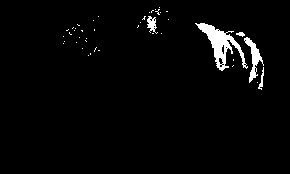
\includegraphics[width=\linewidth]{p7/results/mask_rgb.jpg}
    \caption{RGB-based mask}
  \end{subfigure}\hfill
  \begin{subfigure}[t]{.48\textwidth}
    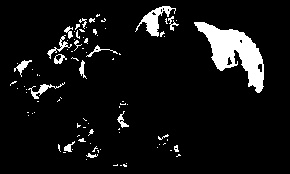
\includegraphics[width=\linewidth]{p7/results/mask_hsi.jpg}
    \caption{HSI-based mask}
  \end{subfigure}
  \begin{subfigure}[t]{.7\textwidth}
    \centering
    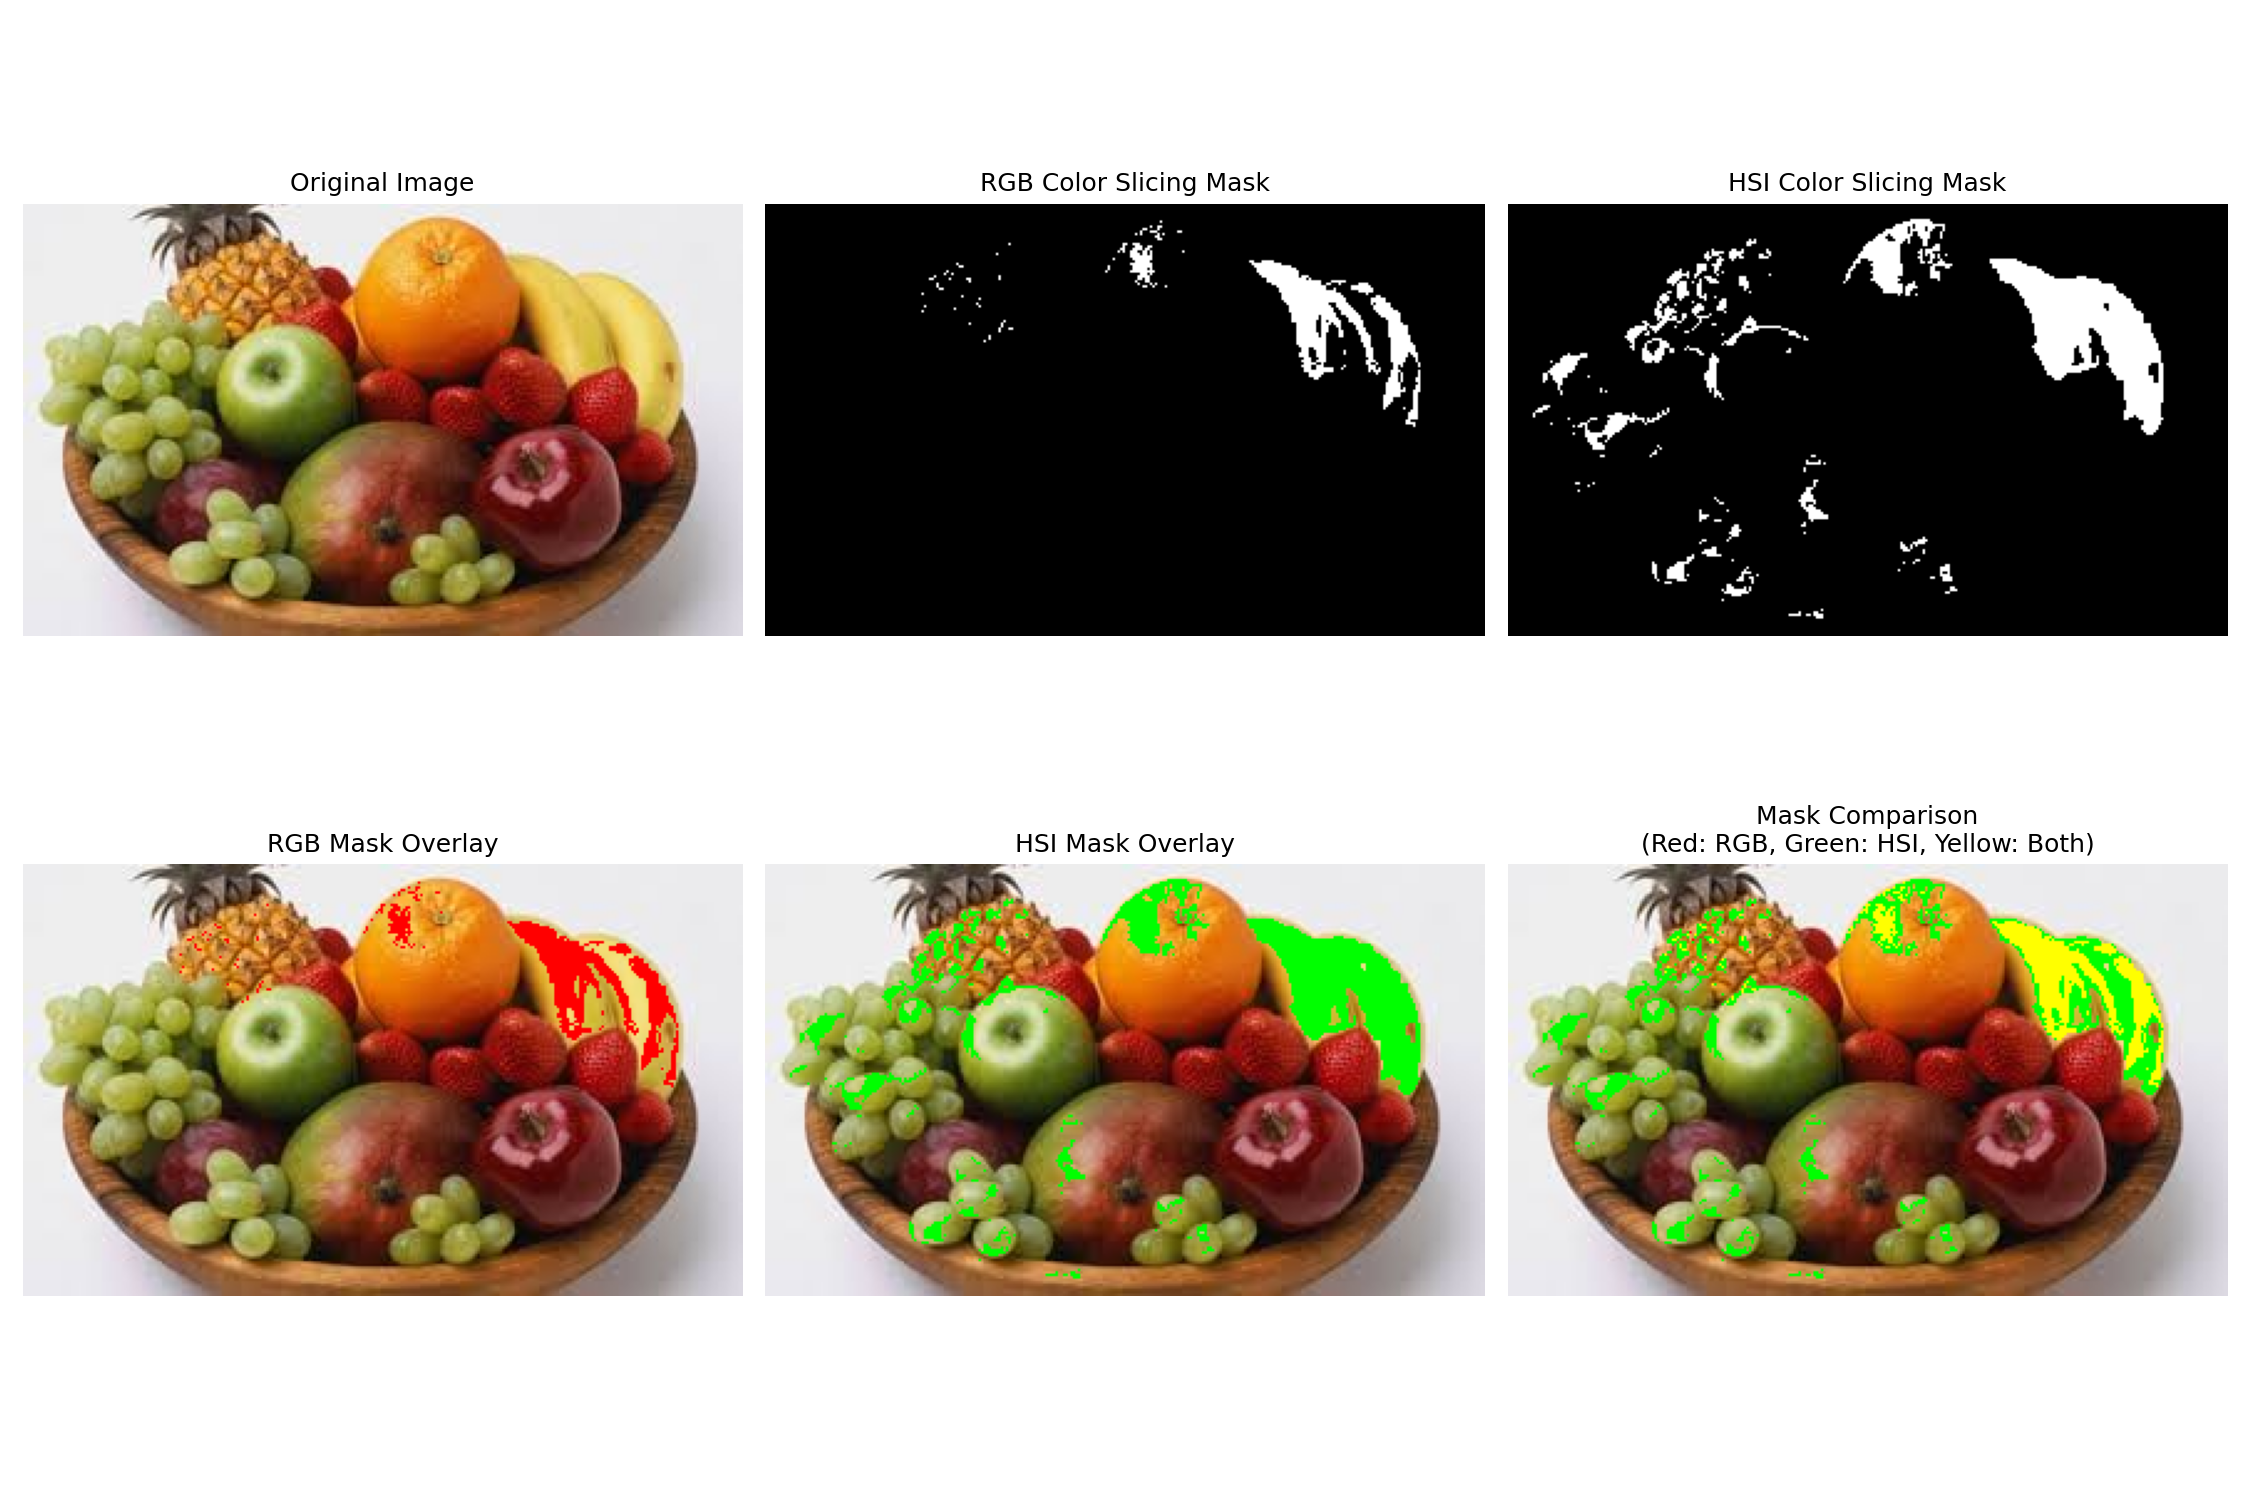
\includegraphics[width=.98\linewidth]{p7/results/mask_comparison.png}
    \caption{Side-by-side comparison}
  \end{subfigure}
\end{figure}

\subsection{C. Transformations}
Additive and multiplicative hue rotations applied to masked regions; summary montage below.

\paragraph{Design goals.}
A realistic recolouring should change the object's perceived hue while preserving texture, shading and natural appearance. This means (a) handling hue as an angular quantity, (b) avoiding abrupt saturation/intensity changes that flatten texture, and (c) applying transformations only on masked pixels (or using a soft mask to blend).

\paragraph{Recommended transform forms.}
Let a source pixel in HSI be $c=(H,S,I)$ and the target colour be $c_t=(H_t,S_t,I_t)$. Common choices:

\begin{itemize}
  \item \textbf{Hue rotation (additive modulo 360):} 
    \[
      H' = (H + \Delta_H) \bmod 360,
    \]
    where $\Delta_H = H_t - H_s$ (often computed from a seed colour $H_s$). Hue must be handled with wrap-around; this is additive (rotation) not multiplicative.
  \item \textbf{Saturation scaling (multiplicative):} 
    \[
      S' = \operatorname{clip}(\alpha_S \cdot S,\,0,1),
    \]
    where $\alpha_S>0$ scales colour purity. Multiplicative change preserves relative differences in saturation across the object.
  \item \textbf{Intensity change (multiplicative or small additive):}
    \[
      I' = \operatorname{clip}(\alpha_I \cdot I + \beta_I,\,0,255),
    \]
    where multiplicative $\alpha_I$ preserves shading contrast (preferred). Small additive $\beta_I$ can be used for uniform brighten/darken but may wash out texture if large.
\end{itemize}

\paragraph{Full per-pixel transform (applied only for mask pixels).}
\[
T(H,S,I) = \big( (H+\Delta_H)\bmod 360,\; \operatorname{clip}(\alpha_S S,0,1),\; \operatorname{clip}(\alpha_I I + \beta_I,0,255) \big).
\]
For a soft mask $w(x,y)\in[0,1]$ blend between original and transformed HSI (or convert back to RGB and blend there):
\[
C_{\text{out}} = (1-w)\,C_{\text{orig}} + w\,C_{\text{transformed}}.
\]

\paragraph{Why additive for hue and multiplicative for S,I?}
Hue is an angular attribute — shifting colour is naturally expressed as an additive rotation on the angle. Saturation and intensity represent magnitudes; multiplicative scaling preserves relative contrast and texture (e.g. shadows remain darker than highlights after scaling). A vector-style multiplicative transform $(c_t / c_s)\cdot c$ is not appropriate because hue is angular and division is undefined when any component is near zero; it also tends to distort chromatic relationships.

\paragraph{Implementation notes and examples.}
\begin{verbatim}
  # Given mask (binary or soft) and transform params:
  delta_H = target_H - seed_H
  alpha_S = desired_saturation_scale  # e.g., 1.2 to increase
  alpha_I = desired_intensity_scale   # e.g., 1.05
  beta_I  = desired_intensity_offset  # e.g., 0

  for each pixel p:
      if mask[p] > 0:
          H' = (H[p] + delta_H) % 360
          S' = clip(alpha_S * S[p], 0, 1)
          I' = clip(alpha_I * I[p] + beta_I, 0, 255)
          out[p] = HSI_to_RGB(H', S', I')
      else:
          out[p] = orig[p]
  # For soft masks, blend out[p] with orig[p] by mask weight.
\end{verbatim}

\paragraph{Qualitative outcomes.}
Using hue rotation with mild saturation scaling and small multiplicative intensity adjustment produces realistic recolouring: the object acquires the new hue while preserving internal shading and texture. Aggressive saturation or intensity changes produce a synthetic, flattened look. When the object contains low-saturation regions, consider applying a reduced hue shift there or increasing saturation first.

\begin{figure}[H]
  \centering
  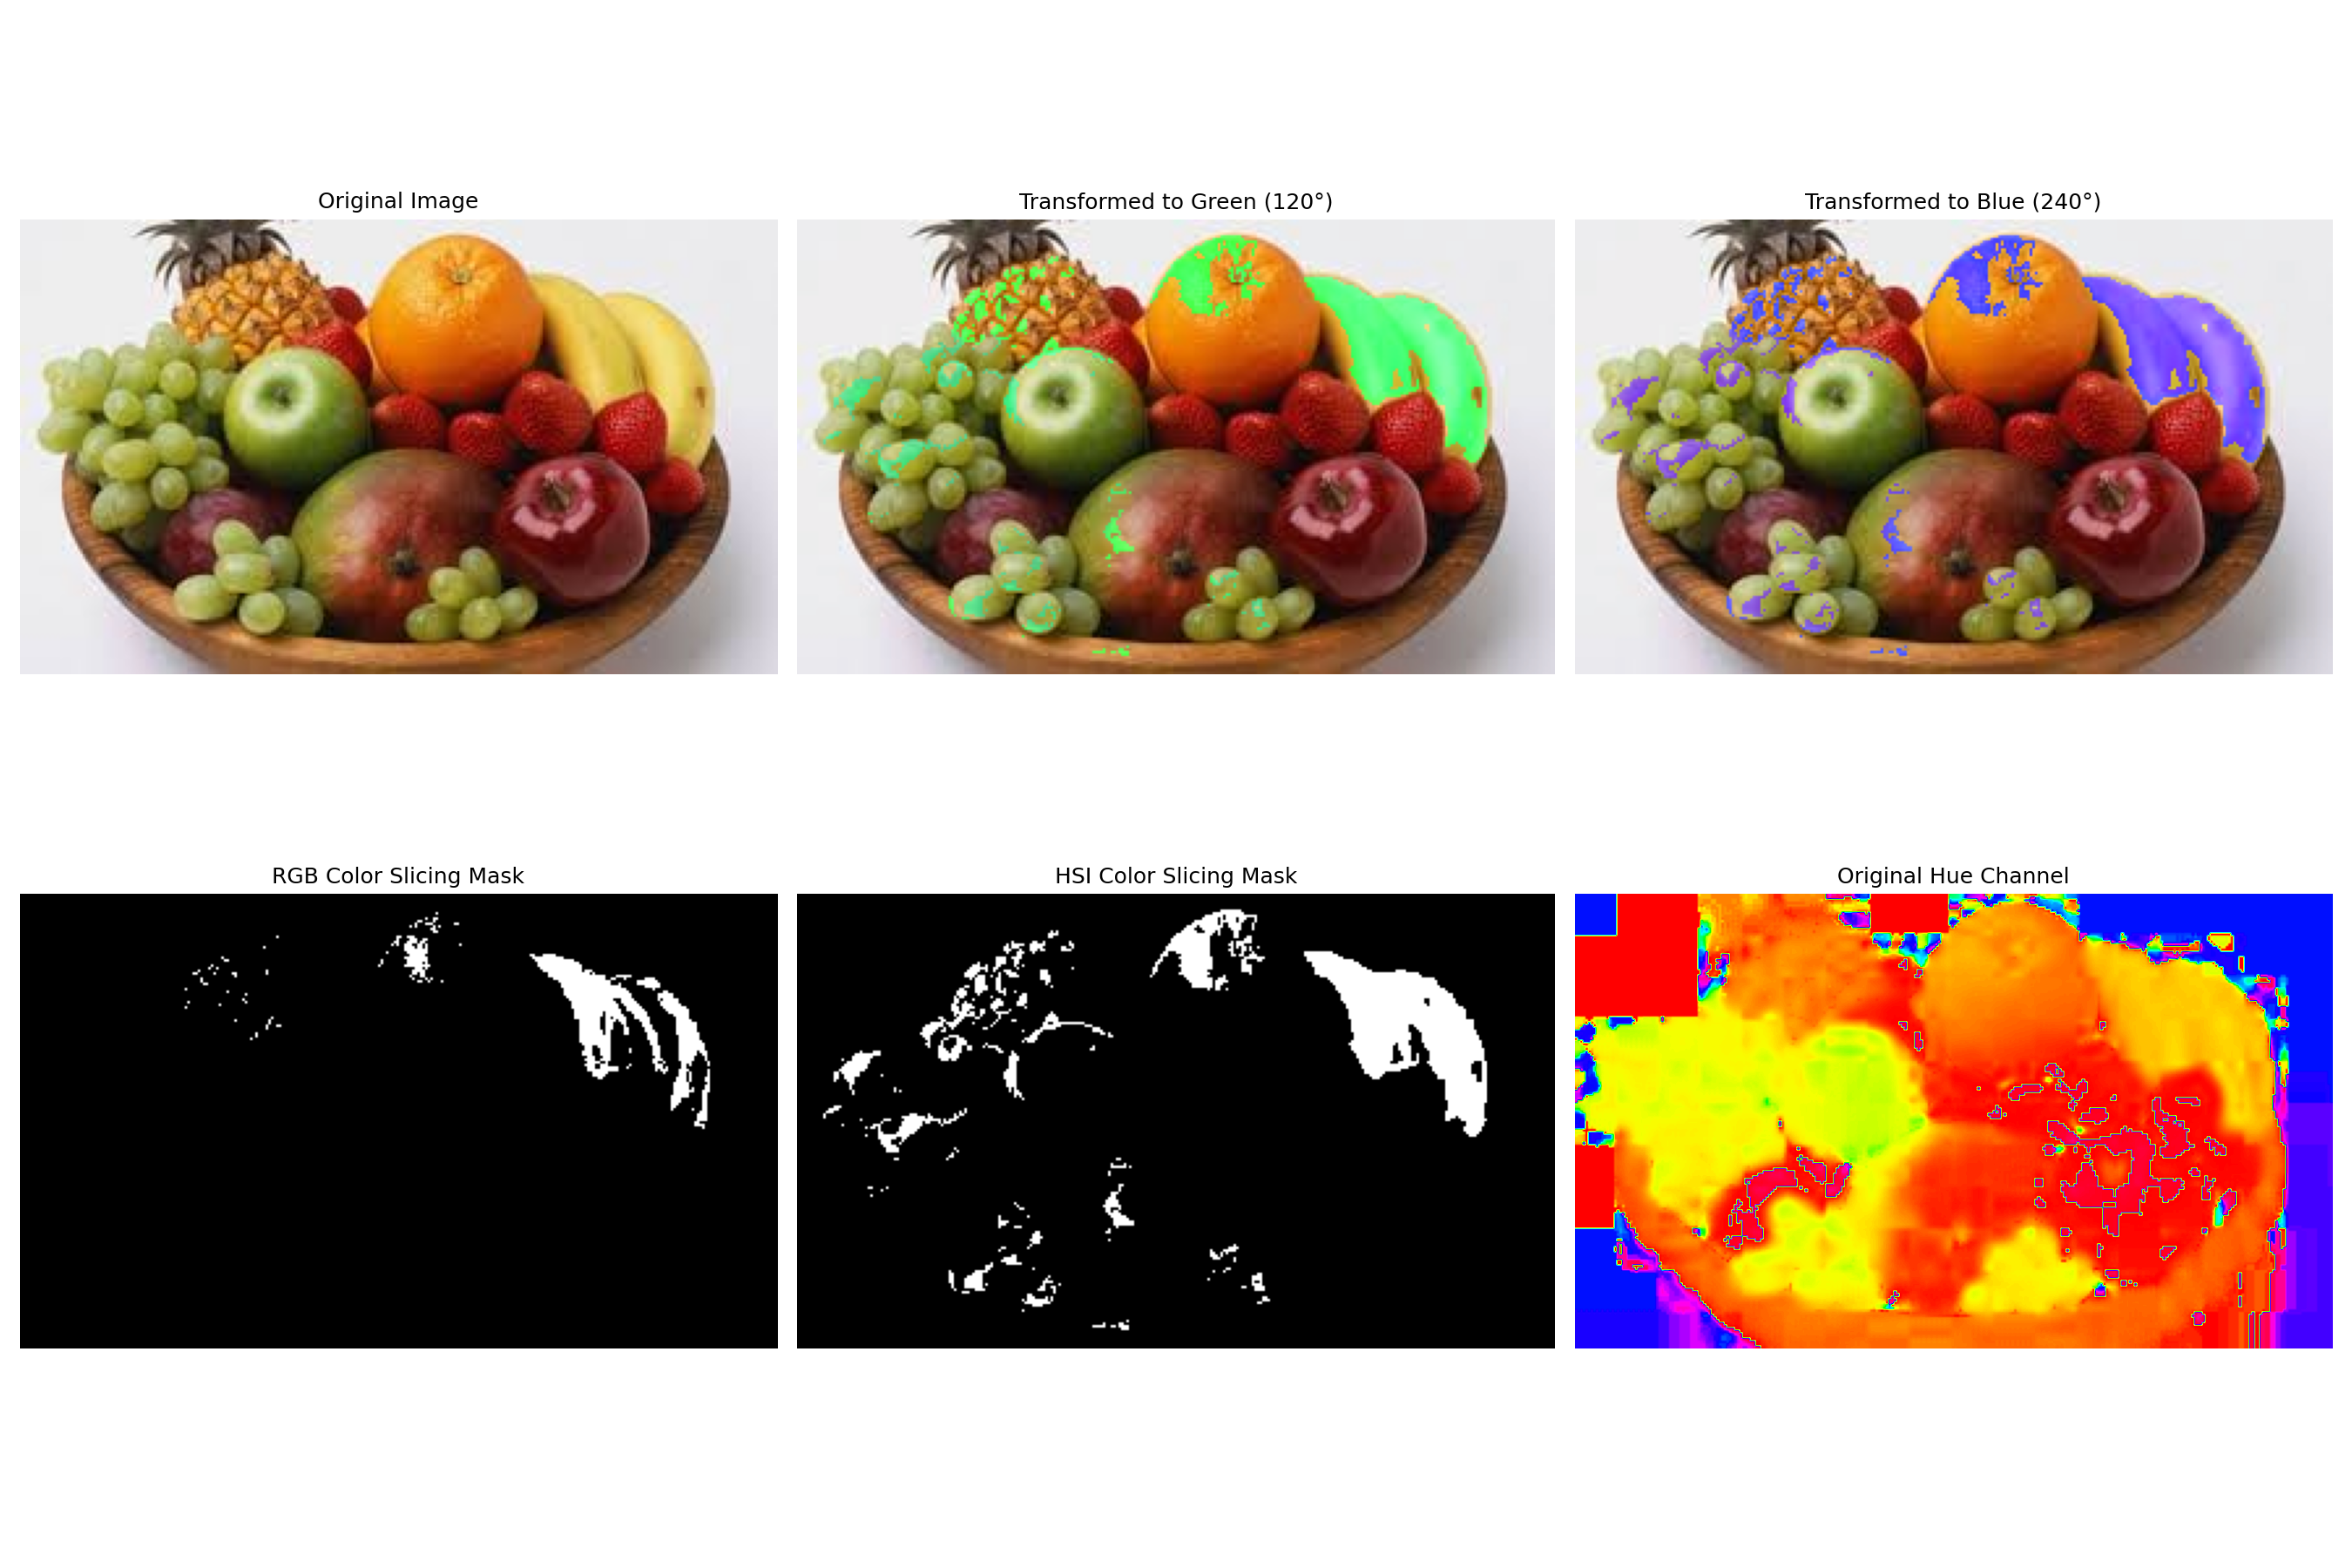
\includegraphics[width=.95\textwidth]{p7/results/transformation_results.png}
  \caption{Representative color-slicing transformations.}
\end{figure}

\end{document}
